\documentclass[deutsch]{lib/llncs/llncs}
\usepackage{lib/llncs/llncsdoc}
\usepackage[ngerman]{babel}
\usepackage[utf8]{inputenc}
\usepackage{hyperref}
\usepackage{graphicx}
\usepackage{lib/picins/picins}
\usepackage[nottoc]{tocbibind}


\begin{document}
\markboth
{Herausforderungen des Zero-Downtime Deployments}
{Herausforderungen des Zero-Downtime Deployments}
\thispagestyle{empty}


\begin{flushleft}
\LARGE\bfseries Herausforderungen des Zero-Downtime Deployments


\end{flushleft}
\rule{\textwidth}{1pt}
\vspace{2pt}


\begin{flushright}
\Huge


\begin{tabular}{@{}l}
Seminar: Problemlösung und Diskussion\\\\
Wintersemester 2017/2018\\\\
Frank Dreyer\\
Matrikelnummer: 741827\\\\
13.03.2018\\[6pt]
\end{tabular}


\end{flushright}
\rule{\textwidth}{1pt}
\vfill

\newpage
\tableofcontents
\newpage\vspace{2pt}


\section{Abstract}
\textit{Continuous Delivery} und \textit{Continuous Deployment} sind wichtige Strategien in der Webentwicklung um Software-Änderungen,  wie zum Beispiel die Behebung eines Bugs oder die Einführung eines Features, schnell auszuliefern und die Anwendung aus dem resultierenden Feedback kontinuierlich verbessern zu können. Eine Schlüsselqualifikation jener Strategien ist trotz regelmäßiger Auslieferungen hochverfügbar zu bleiben. \\
Dieser Beitrag beschäftigt sich mit der Frage wie Software-Auslieferungen durchgeführt werden können ohne die Anwendung temporär abschalten zu müssen. \\
Dafür werden zunächst einige Auslieferungsstrategien, wie z.B. das Blue Green Deployment oder Carnary Releases, gegenübergestellt. Daraufhin wird auf die Herausforderung der Datenbank-Migration genauer eingegangen und \textit{QuantumDB}, ein Tool zur Lösung dieser Problematik, vorgestellt und evaluiert. 


\newpage


\section{Einleitung}


\section{Die Wahl der Auslieferungsstrategie}
Eine Herausforderung bei der Auslieferung von Änderungen ohne auf den Dienst der Anwendung verzichten zu müssen, ist die Wahl der Auslieferungsstrategie. Diese muss so organisiert sein, dass zur neuen Version der Anwendung ohne Zeitverzögerung umgeschaltet werden kann. Sollte es nach Auslieferung zu Komplikationen der neuen Version kommen (z.B. durch einen schwerwiegenden Bug in einem neuen Feature), sollte es außerdem möglich sein zur alten, stabilen Version umgehend zurückspringen zu können. Des weiteren kann es unter Umständen notwendig sein beide Versionen, die alte wie auch die neue, gleichzeitig einzusetzen.\\
Nachfolgend werden einige Strategien vorgestellt, die sich dieser Herausforderungen widmen und einen Austausch von Softwarekomponenten ohne Ausfallzeit ermöglichen. 


\subsection{Blue-Green Deployments}
Beim \textit{Blue-Green Deployment} gibt es sowohl eine blaue als auch eine grüne Instanz einer Produktionsumgebung, die möglichst identisch sein sollten. Zu jeder Zeit ist eine der Produktionsumgebungen aktiv während die andere inaktiv ist. Soll nun eine Änderung durchgeführt werden, etwa durch ein neues Feature in einer Anwendung, so wird diese Änderung bei der inaktiven Produktionsumgebung umgesetzt, ohne die aktive abschalten zu müssen. Im Anschluss wird die aktualisierte Produktionsumgebung ausgiebig getestet, bevor getauscht und der Datenverkehr fortan zur neuen aktiven Produktionsumgebung geleitet werden kann, während die alte inaktiv wird. \\
Sollte es trotz präventiver Tests zu unerwarteten Komplikationen beim Einsatz der neuen Produktionsumgebung kommen, so bietet sich durch \textit{Blue-Green Deployments} immer die Möglichkeit die alte Version wiederherzustellen, indem der Datenverkehr zur Vorgängerumgebung zurückgelenkt wird und aktive und inaktive Umgebung erneut tauschen. Die Rolle des Umschaltens kann dabei von einer Routing-Komponente übernommen werden, die je nach Konfiguration den Datenverkehr entweder zur einen oder anderen Produktionsumgebung weiterleitet. Abbildung 1 illustriert den klassischen Aufbau der Komponenten eines \textit{Blue-Green Deployments}. 	
\begin{figure}
	\centering
	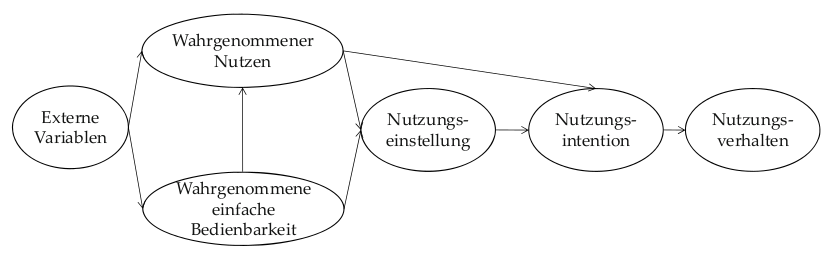
\includegraphics[scale=0.40]{img/abbildung1.png}
	\caption{\textit{Technology Acceptance Model} (Vgl. \cite[S. 237]{bandow2010modell})}
\end{figure}




\bibliographystyle{alphadin}
\bibliography{lit/lit}


\end{document}
